%%%%%%%%%%%%%%%%%%%%%%%%%%%%%%%%%%%%%%%%%%%%%%%%%%%%%%%%%%%%%%%%%%%%%%%%
% Plantilla TFG/TFM
% Escuela Politécnica Superior de la Universidad de Alicante
% Realizado por: Jose Manuel Requena Plens
% Contacto: info@jmrplens.com / Telegram:@jmrplens
%%%%%%%%%%%%%%%%%%%%%%%%%%%%%%%%%%%%%%%%%%%%%%%%%%%%%%%%%%%%%%%%%%%%%%%%

\chapter{Diseño y análisis de arrays de parches microstrip}
\label{diseño}

\section{Introducción}

\par En este capítulo se va a abordar la realización del diseño inicial de un conjunto de configuraciones de arrays de antenas microstrip para las frecuencias de 2.4 Ghz, 6 Ghz y 27 Ghz. Como se mencionó en la sección \ref{sec:medodologia}, el diseño y simulación de estas configuraciones se realizará mediante la herramienta Ansys \sffamily\textregistered  HFSS y MathWorks \sffamily\textregistered  MATLAB.
\\
\par Todos las antenas de parche microstrip individuales y las posibles configuraciones de array que se diseñen con el conjunto de estas, estarán basadas en unos criterios y especificaciones de construcción común:

\begin{itemize}
	\item \textbf{Polarización: }Lineal
	\item \textbf{Tipo de alimentación: } Directa por línea microstrip
	\item \textbf{Impedancia de entrada: }50 $\Omega$
	\item \textbf{Altura del substrato: }1.52 \SI{3.55}{\milli\metre}
	\item \textbf{Altura de los planos conductores: }\SI{3.55}{\micro\metre}
	\item \textbf{Substrado: }Rogers 4003 (RO4003)
	\item \textbf{Constante dieléctrica del substrato: }3.55
\end{itemize}

\section{Cálculos iniciales con MATLAB}
\par En primer lugar, se realizará un síntesis de las ecuaciones necesarias para diseñar parches microstrip en MATLAB. Para ello usaremos las ecuaciones recogidas en la sección \ref{analisis}. Se explicará paso a paso el código implementado para la obtención de estos resultados.
\\
\par En primer lugar se realizará la declaración inicial de variables, donde se almacenarán en la memoria del computador los valores de las constantes que se usarán a lo largo de los cálculos. La única variable que tendrá que ser introducida a mano por el usuario es la frecuencia en Ghz a la que se desea realizar el diseño de la antena. Además, desde aquí se realizará el cálculo de otros parámetros que necesitaremos más adelante, como la longitud de onda \textit{$\lambda_{0}$} o el número de onda \textit{k}.

\begin{lstlisting}[style=Matlab-color, caption={Declaración de variables iniciales},label=variniciales]
%% Input Variables
f = input('Introduzca la frecuencia de trabajo deseada (Ghz): ');   % Frecuencia a la que se vana a realizar los cálculos

er = 3.55;										% Constante dieléctrica
h = 1.52;										% Altura del substrato

% Otras variables
c = physconst('LightSpeed');					% Velocidad de la luz
f = f*1e9;										% Frecuencia en Ghz
h = h*1e-3;										% Longitud en mm
lambda = c/f;									% Longitud de onda en el vacío
ko = 2*pi/lambda;								% Número de onda
Zo = 50;										% Impedancia de entrada
\end{lstlisting}

\par A continuación se procederán calcular los parámetros característicos del diseño de la antena como son su anchura \textit{W}, longitud \textit{L}, etc. 

\begin{lstlisting}[style=Matlab-color, caption={Parámetros de diseño de la antena},label=diseñoantena]
%% Cálculos del Parche

W = (c/(2*f))*sqrt(2/(er+1));                       % Ancho del Parche (Width)
erff = ((er+1)/2) + ((er-1)/2)*(1+12*h/W)^(-1/2);   % Coeficiente del dieléctrico efectiva
Leff = c/(2*f*sqrt(erff));                          % Longitud efectiva
Al = ((0.412*h*(erff+0.3)*((W/h)+0.264))/((erff-0.258)*((W/h)+0.8))); % Incremento de Longitud normalizada
L = Leff - 2*Al;                                    % Longitud del parche
a = 0.7*lambda;                                     % Separacion entre parches
\end{lstlisting}

\par También calcularemos la anchura $W_{feed}$ y longitud $L_{feed}$ necesaria para las líneas de transmisión microstrip así como la longitud para las líneas que actúen como transformadores $\lambda /4$. La anchura de las líneas microstrip será calculada en base a la variable $Z_{0}$, la cual ha sido declarada anteriormente con un valor de 50 ($\Omega$), este valor puede ser cambiado en el código para obtener la anchura de la línea para sintetizar cualquier impedancia que necesitemos en esta.

\begin{lstlisting}[style=Matlab-color, caption={Parámetros de diseño de la línea de alimentación},label=alimentacion]
%% Cálculos de línea de alimentación

lambdaguided = lambda/sqrt(erff);               % Longitud de onda en medio guiado
Lfeed = lambdaguided/4;                         % Longitud lambda cuartos

%Calculo de la anchura de la línea
A = (Zo/60)*(sqrt((er+1)/2))+((er-1)/(er+1))*(0.23+(0.11/er)); 
B = (377*pi)/(2*Zo*sqrt(er));
Coef = (8*exp(A))/((exp(2*A))-2);
if (Coef <= 2)
	Wline = Coef*h;                             % Anchura si W/h <= 2
elseif (Coef > 2)
    Coef = (2/pi)*( B-1-log(2*B-1)+((er-1)/(2*er))*(log(B-1)+0.39-(0.61/er)));
	Wline = Coef*h;                             % Anchura si W/h > 2
end
\end{lstlisting}

\par Finalmente, se calculará la longitud que deberán tener las ranuras o \textit{insets} para adaptar que la línea de alimentación encuentre la posición dentro de la antena donde se adaptan sus impedancias.

\begin{lstlisting}[style=Matlab-color, caption={Parámetros de diseño del \textit{inset}},label=inset]
%% Inset

I1 = @(theta) (sin((ko*W/2)*cos(theta))./cos(theta)).^2.*sin(theta).^3;
G1 = integral(I1,0,pi)/(120*pi^2);          % Admitancia de la TL
I2 = @(theta) ((sin((ko*W/2)*cos(theta))./cos(theta)).^2).*besselj(0,ko*L*sin(theta)).*sin(theta).^3;
G12 = (1/(120*pi^2)).*integral(I2,0,pi);        % Admitancia mutua
Rin = 1./(2*(G1+G12));                          % Impedancia de entrada
yo = (L/pi).*acos(sqrt(Zo/Rin));        % Longitud del inset
\end{lstlisting}

\par Con todos estos parámetros calculados se podrá proceder a diseñar y analizar los arrays de antenas en HFSS.

\section{Diseño y Análisis en Ansys HFSS}

\par Es el momento de comenzar con el diseño de las antenas y los arrays de antenas en tecnología micorstrip mediante Ansys HFSS. Se han escogido una serie de configuraciones a diseñar que varían desde un solo elemento hasta un array compuesto de 16 elementos en disposición de array bidimensional. De esta manera, podrá analizarse al final del proyecto, qué tipo de configuración es la más adecuada para nuestras características, en conceptos como directividad, patrón de radiación, eficiencia o dimensiones.
\\
\par Las configuraciones elegidas son las siguientes:

\begin{itemize}
\item Antena de parche de un único elemento
\item Array de parches \textbf{2x1} (2 antenas) dispuestas en serie
\item Array de parches \textbf{2x1} (2 antenas) dispuestas en paralelo
\item Array de parches \textbf{2x2} (4 antenas) dispuestas en paralelo
\item Array de parches \textbf{4x1} (4 antenas) dispuestas en paralelo
\item Array de parches \textbf{4x2} (8 antenas) dispuestas en paralelo
\item Array de parches \textbf{4x4} (16 antenas) dispuestas en paralelo
\end{itemize}

\par Estas configuraciones serán repetidas en diferentes análisis para las frecuencias de: \textbf{2.4 GHz}, frecuencia usada para aplicaciones comunes como \gls{wifi} o Bluetooth, donde la cobertura es uno de los principales factores de calidad en su uso. \textbf{6 GHz}, banda prevista para el despliegue de redes 5G de alta velocidad en el futuro. Y \textbf{27 GHz}, banda ya adjudicada para aplicaciones 5G de ultra-rápida velocidad y mínima latencia. Para este último caso, solo se realizará el diseño para el caso de una antena parche de un único elemento \todo{camviar si hago ams}
\\
\par Antes de empezar con el diseño, se va a proceder a mencionar ciertos parámetros de configuración de la herramienta Ansys HFSS, los cuales son necesarios a tener en cuenta para entender los resultados obtenidos, así como a explicar ciertos conceptos básicos sobre el funcionamiento de HFSS y realizar paso por paso, como ejemplo, el diseño de la antena parche básica.

\subsection{Consideraciones previas de Ansys HFSS}

\par Las consideraciones previas en cuanto a configuración y diseño en común a todas las antenas a diseñar son:
\\
\par Todos los diseños serán realizados en el plano XY, donde el eje Y estará dedicado a las alturas y el eje X a las anchuras. La alimentación de la línea de transmisión será realizada mediante la técnica denominada Wave-port. Mediante los wave-port HFSS asume que la alimentación del sistema esta siendo realizada por una guía de onda semi-infinita cuya sección y propiedades son las mismas que se le asignen a este wave-port. A la hora de realizar el análisis de los parámetros de pérdidas de retorno (S), HFSS asume que el wave-port excitará el sistema con los modos naturales asociados a la sección de esa guía de onda. Cada modo con el que se excita el puerto contiene un vatio de potencia. Por otra parte, los parámetros S serán referenciados a la impedancia que le sea asignada a este puerto en el momento de su declaración en el programa, en nuestro caso 50 $\Omega$.
\\
\par Los planos conductores, es decir, el conjunto de parche y alimentación y el plano de tierra tendrán la propiedad de \textit{PerfectE}, lo que le proporciona las características de superficie conductora perfecta. A esta propiedad también se le denomina \textit{boundary} y no ha de confundirse con el material asignado a los elementos conductores. Esta propiedad obliga al campo eléctrico a ser perpendicular a la superficie. Otro \textit{boundary} o contorno esencial que encontraremos en nuestros diseños es el \textit{Radiation}. La propiedad \textit{boundary} de \textit{radiation}, la cual será asignada a la caja de radiación que rodee el sistema completo en sus tres dimensiones, será capaz de simular la propagación de la radiación a una distancia infinita, pudiendo analizar así nuestra antena como si nos encontráramos en la región de campo lejano.
\\
\par En cuanto a los materiales asignados a cada elemento, la configuración será la misma para todos los diseños: La caja de radiación será asignada a vacío, así asumiremos que no hay ningún tipo de pérdidas de propagación a la hora de realizar el análisis. El substrato será asignado a \textit{Rogers RO4003}, diseñado para circuitos de alta frecuencia y fabricado con láminas de cerámicas de hidrocarburos, cuya constante dieléctrica $\varepsilon_{r}$ es de 3.55, y su factor de pérdidas $\tan \delta$ es de 0.0021 a 2.5 GHz.
\\
\par El proceso de análisis que realiza HFSS para simular el comportamiento eléctrico de los diseños se basa en el \gls{fem} o método de elementos finitos. Para ello, HFSS crea una malla de tetraedros a lo largo de las diferentes superficies de nuestro diseño. HFSS irá realizando iteraciones de la simulación donde en cada una de ellas, los tetraedros irán reduciendo su tamaño y adaptándose automáticamente a la forma de nuestro diseño. De esta forma, nuestro diseño es discretizado y en cada uno de estos tetraedros serán calculadas las ecuaciones de Maxwell en forma diferencial. En cada iteración se compararán los resultados obtenidos en cuanto a la dispersión de los puertos con la iteración anterior, la diferencia entre ambas comparaciones se denominará \textit{delda S}. Cuanto mayor sea este parámetro, mayor diferencia entre los resultados de las iteraciones, lo que significará que nuestro análisis aun necesita realizar más iteraciones, en las que los tetraedros se adapten del todo con el diseño, de forma que no exista variación de los resultados entre iteraciones.
\\
\par Para ello, a la hora de configurar el \textit{solver}, en nuestras simulaciones hemos elegido un número máximo de pasadas de 30, el cual siempre ha sido suficiente para que las simulaciones llegaran a converger y un valor de error de convergencia, \textit{delta S}, de 0.002. Cuanto menor sea el valor, más precisos serán los resultados obtenidos, y por tanto, mayores cálculos tendrá que realizar nuestro computador. Este ha sido importante a la hora de realizar el proyecto, puesto que, no siempre se ha podido simular con tanta precisión debido a las limitaciones de la computadora en la que se está trabajando, con lo que se ha tenido que llegar a una solución de compromiso para el caso de los diseños más complejos: El array de 4x2 y de 4x4. En estos casos hemos tenido que aumentar la convergencia hasta valores de 0.02, puesto que simulaciones con menor convergencia llevaban al proyecto de HFSS a tardar varios días en completarse.
\\
\par Otro ajuste previo a la simulación en HFSS es el \textit{Frequency sweep} o barrido en frecuencia. Con el se ajustará cual será el margen de frecuencias para el que se realizarán los cálculos de la simulación. En nuestro caso siempre será en un margen de $\pm$ 0.1 GHz con respecto a la frecuencia a la que se va a realizar la simulación. Este valor es suficiente para poder observar la curva de pérdidas de retorno completa para esta frecuencia. Además, se puede ajustar el intervalo de discretización del eje de frecuencias, para poder obtener así una mayor resolución en las gráficas que se vayan a analizar. En nuestro caso se ha elegido un intervalo de 0.0001. Por ejemplo, si nuestra frecuencia de diseño es de 2.4 GHz, la gráfica se mostrará desde los 2.3 GHz hasta los 2.5 GHz, cada 0.00001 GHz, lo que nos dará un total de 2001 puntos de resolución.
\\
\par Para el análisis de los resultados, nos basaremos principalmente en las gráficas y parámetros que HFSS nos ofrece. Usaremos los reportes de las soluciones modales para graficar las pérdidas de retorno o parámetros S y comprobar así el ancho de banda, la frecuencia de trabajo y la calidad de nuestra antena. También nos fijaremos en las gráficas que analizan la parte real e imaginaria (óhmica y reactiva) de la impedancia, para así conocer el grado de adaptación de las impedancias de nuestra antena. 
\\
\par En cuanto a los reportes sobre el campo lejano de la antena, analizaremos los patrones de radiación 2D para los dos planos de radiación de la antena, E y H, es decir, cuando $\phi $ = 0º y $\phi $ = 90º y el diagrama de radiación polar en 3D, en ambos casos se mostrará la directividad de la antena en dBs. Otras características que HFSS ofrece para analizar el comportamiento de la antena, y que también se usarán en este proyecto, es la representación sobre la antena del comportamiento de los campos eléctrico y magnético, así como la visualización de los tetraedros usados por HFSS para analizar la antena. Para terminar, usaremos la HFSS para calcular automáticamente los valores de los parámetros característicos de la antena tales como directividad, eficiencia, etc.
\\
\par Finalmente, cabe mencionar que todos los diseños estarán parametrizados. Esto quiere decir que cada parámetro de anchura y altura de cualquier sección del conjunto del parche estará asociado a una variable o a la derivación del cálculos entre otras variables. Se ha seguido una serie de patrones a la hora de declarar estas variables de forma que sea sencillo entender a qué sección pertenece cada una:

\begin{itemize}
\item \textbf{W/L: }Anchura/Altura del parche
\item \textbf{Ws/Ls: }Anchura/Altura del substrato
\item \textbf{Wwp/Lwp: }Anchura/Altura del \textit{Waveport}
\item \textbf{h: }Grosor del substrato
\item \textbf{Linset/Winset: }Anchura/Altura del \textit{inset}
\item \textbf{W50/L50: }Anchura/Altura para línea con impedancia de 50 $\Omega$
\item \textbf{W100/L100: }Anchura/Altura para línea con impedancia de 100 $\Omega$
\item \textbf{W70/L70: }Anchura/Altura para línea con impedancia de 70.71 $\Omega$
\item \textbf{W25/L25: }Anchura/Altura para línea con impedancia de 25 $\Omega$
\end{itemize}

\par En caso de que se necesiten otras variables estás tendrán una codificación del tipo: "Xdesc". Donde \textit{X} es W o L según si la variable referencia a una anchura o a una altura respectivamente y \textit{desc} será una palabra corta o acrónimo que defina el objeto al que hace referencia, por ejemplo: \textit{feed}.


\subsection{Proceso de diseño en HFSS}
\par A continuación se va a explicar detenidamente el proceso de diseño y configuración de HFSS para el caso de la antena de parche única a 2.4 GHz, así como a analizar los resultados obtenidos. Para ello empezaremos usando el script diseñado en MATLAB anteriormente mostrado. Los resultados obtenidos son los que serán usados en HFSS para diseñar la primera aproximación de la antena. En este caso:

\begin{table}[H]
   
   \label{tab:antena1x12}
   \small % text size of table content
   \centering % center the table
   \begin{tabular}{m{0.2\linewidth}m{0.15\linewidth}} % alignment of each column data
   \toprule[\heavyrulewidth]\toprule[\heavyrulewidth]
   \textbf{Parámetro} & \textbf{Dimensión} \\ 
   \midrule
   \textbf{W} & 41.40 mm \\
   \textbf{L} & 32.73 mm \\
   \textbf{Linset} & 11.89 mm \\
   \textbf{Winset} & 1 mm \\
   \textbf{W50} & 3.36 mm \\
   \textbf{Ws/Ls} & 70 mm \\
   \textbf{5} & 1.52 mm \\
   \bottomrule[\heavyrulewidth] 
   \end{tabular}
   \caption{Resumen de dimensiones de parche único microstrip} 
\end{table}

\par Crearemos un nuevo proyecto en HFSS y empezaremos creando un \textit{box}, definiendo las variables que le dará dimensiones y centrándolo en el viasualizador del proyecto. Para ello, como se ha mencionado anteriormente, se usarán las variables creadas o los cálculos derivados de ellas para obtener los resultados deseados (fig. \ref{fig:substrato}). Observaremos que el cubo aparece ahora en la lista de sólidos del proyecto. Desde allí le asignaremos el material que le corresponde mediante la opción \textit{Assign Material}. 
\\
\begin{figure}[h]
    \centering
        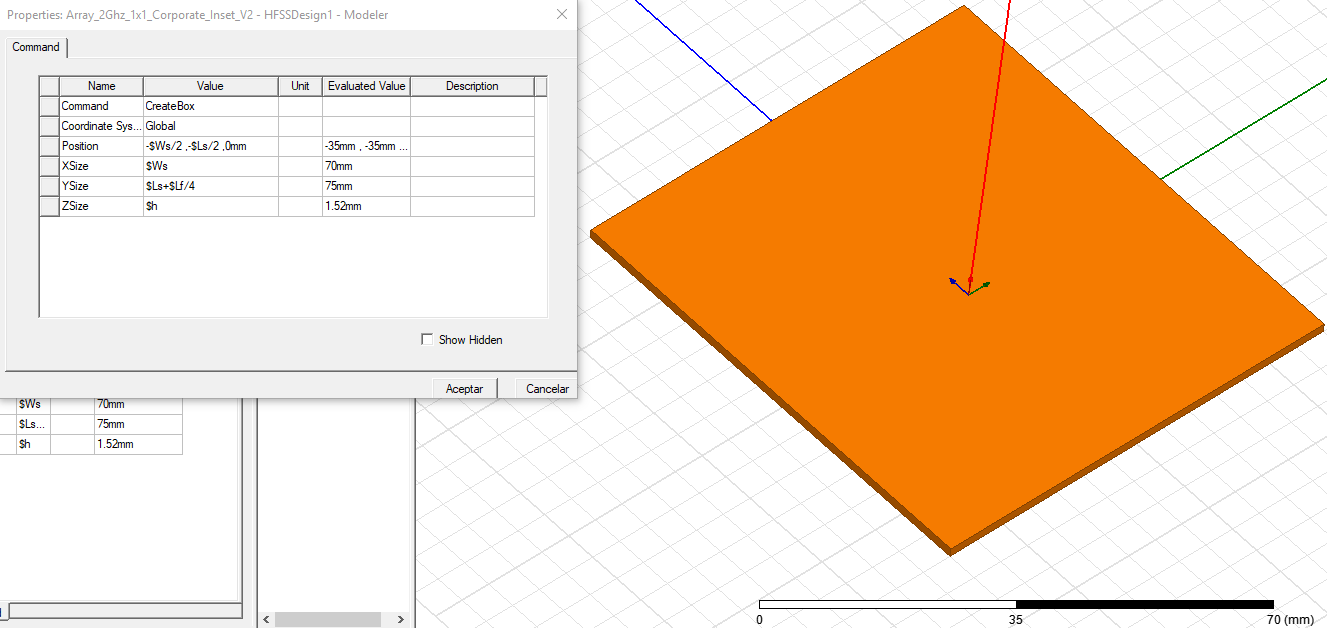
\includegraphics[width=13cm]{archivos/desarrollo/1}
        \caption{Creación del substrato}
        \label{fig:substrato}
\end{figure}
\par El plano de masa se creará mediante un plano simple. Para ello se usará la herramienta \textit{Draw Rectangle}, de igual manera que con el substrato, se le asignarán las variables idénticas a las asignadas al substrato, puesto que ambos tendrán el mismo ancho y alto, y se configurará su posición para que este esté centrado y pegado al plano inferior del substrato (fig. \ref{fig:masa}).
\\
\begin{figure}[h]
    \centering
        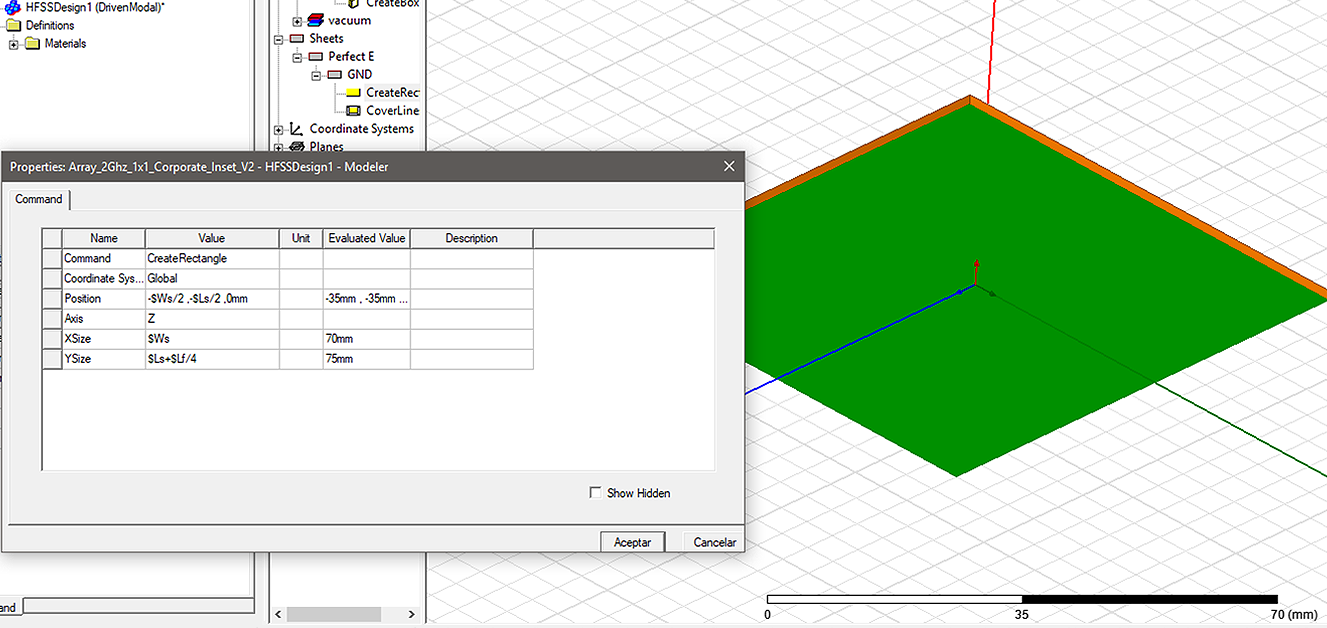
\includegraphics[width=13cm]{archivos/desarrollo/2}
        \caption{Creación del plano de masa}
        \label{fig:masa}
\end{figure}
\par A continuación, se volverá al plano superior del substrato, y volviendo a usar la herramienta \textit{Draw Rectangle} se creará un rectángulo con las medidas de W y L como ancho y alto respectivamente. Este rectángulo será nuestro parche (fig. \ref{fig:parche}). Cabe destacar como, todo lo relacionado con el parche, y el resto de circuitos de alimentación estarán situados sobre el substrato, es decir, a 1.52 mm sobre el origen de coordenadas del diseño del HFSS. Se volverá a repetir el proceso para el feed de alimentación, que unirá en uno de los lados que definen la anchura del parche al lado paralelo más próximo que define el ancho del substrato (fig. \ref{fig:feed}).
\\ 
\begin{figure}[h]
    \centering
        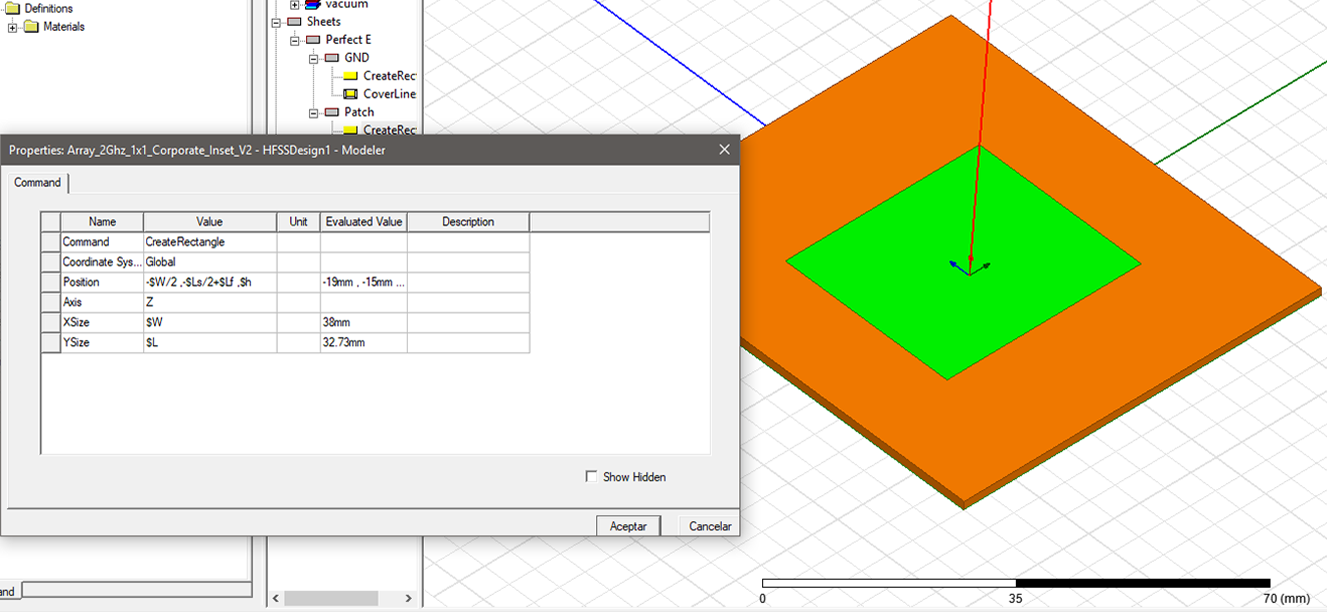
\includegraphics[width=13cm]{archivos/desarrollo/3}
        \caption{Creación del parche}
        \label{fig:parche}
\end{figure}
\begin{figure}[h]
    \centering
        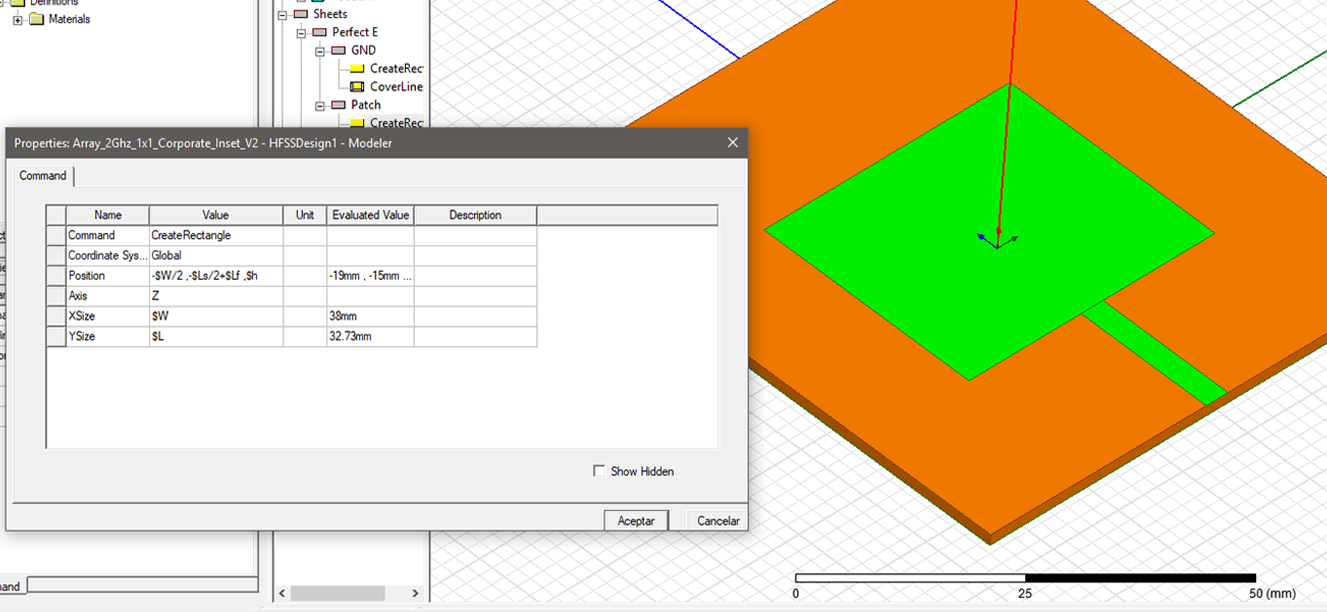
\includegraphics[width=13cm]{archivos/desarrollo/4}
        \caption{Creación del feed principal}
        \label{fig:feed}
\end{figure}
\par Seleccionando ahora los planos correspondientes a el \textit{feed} y el parche se procederá a pulsar el botón \textit{Unite}, que se encargará de unirlos como si fuera un solo material. Con este nuevo sólido que se habrá creado y seleccionando simultáneamente el rectángulo creado para el plano de masa se accederá a sus opciones y se pulsará sobre la opción \textit{Assign Boundary}>\textit{Perfect E}. De esta forma le daremos el comportamiento de conductor perfecto al conjunto de \textit{feed} y parche y al plano de masa (fig. \ref{fig:perfecte}). 
\\
\begin{figure}[h]
    \centering
        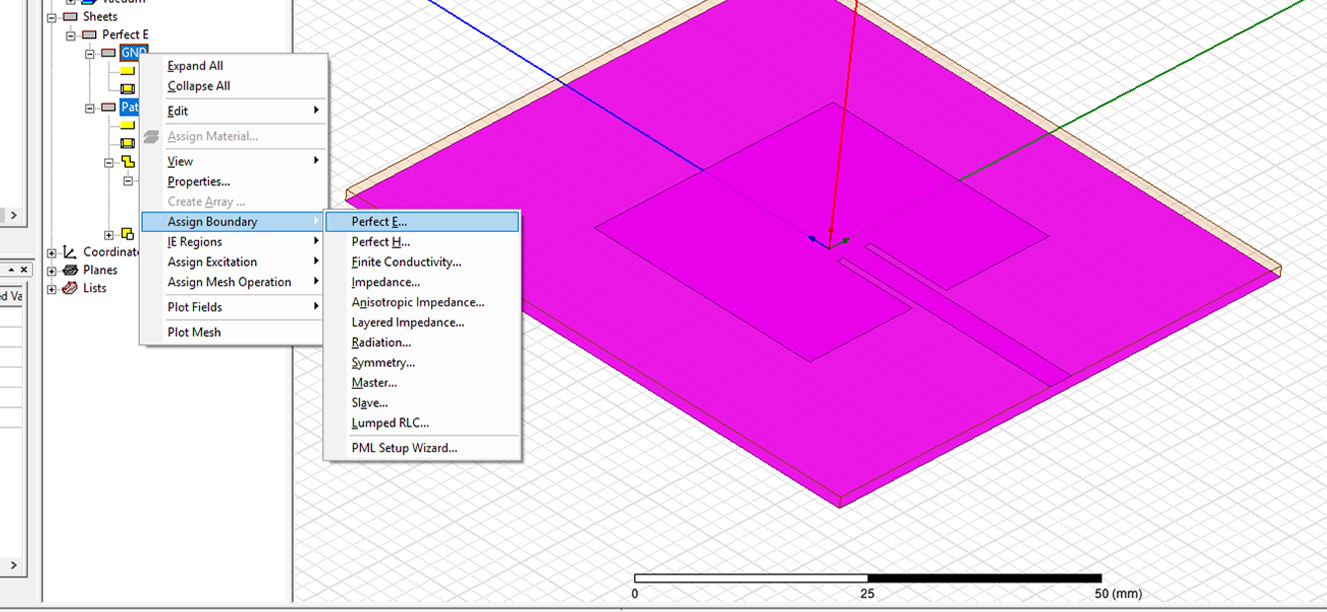
\includegraphics[width=13cm]{archivos/desarrollo/5}
        \caption{Asignación de material conductor al parche y al plano de masa}
        \label{fig:perfecte}
\end{figure}
\par Para excitar el sistema crearemos el \textit{Wave port}. Para ello se cambiará el plano de diseño de XY a ZX, para poder crear planos perpendiculares a los ya existentes en la antena. El \textit{Wave port} consistirá en un rectángulo que repose centrado sobre el extremo del substrato donde se puede acceder al \textit{feed}. Este debe tener unas dimensiones para cubrir el \textit{feed} por completo, así como tocar el plano de masa (fig. \ref{fig:waveport}). De la misma manera que se usó para asignar la propiedad de conductor al parche, se seleccionará sobre el plano creado para el \textit{Wave port} y en sus opciones aplicaremos: \textit{Assign Excitation}>\textit{WavePort}. 
\\

\begin{figure}[h]
    \centering
        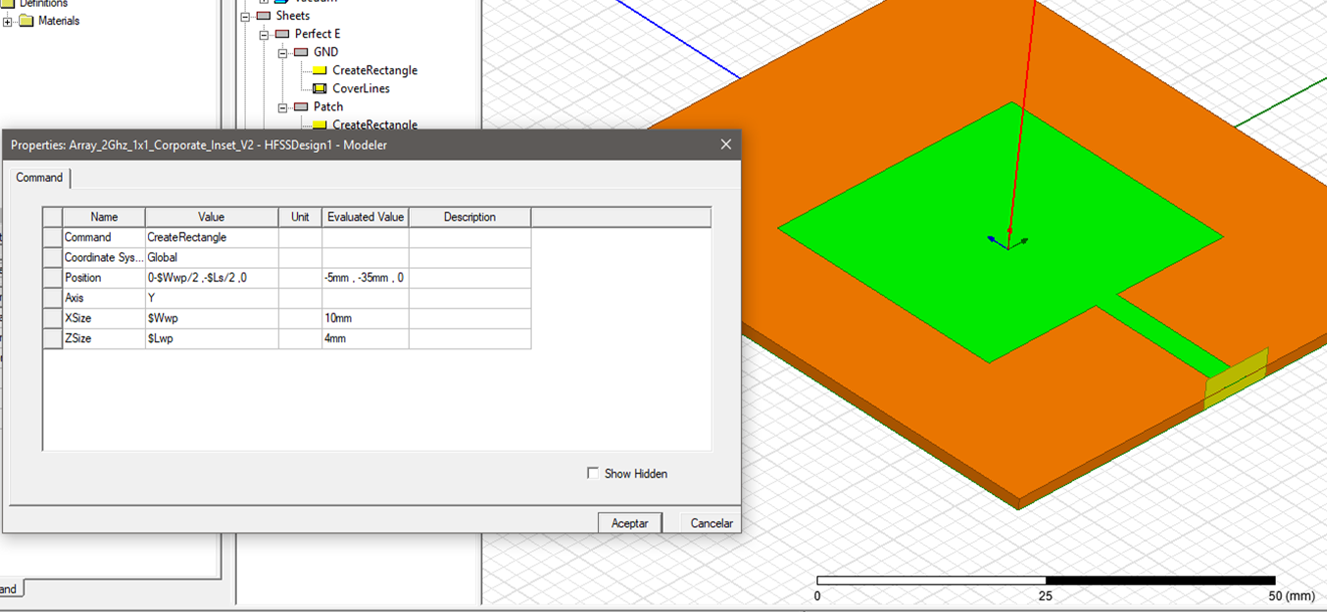
\includegraphics[width=13cm]{archivos/desarrollo/6}
        \caption{Creación del Wave-Port}
        \label{fig:waveport}
\end{figure}

\par Los dos ranuras o \textit{insets} que adaptarán el \textit{feed} y la antena, se crearán como rectángulos sobre el substrato y pegados al \textit{feed} dentro del parche (fig. \ref{fig:inseta}). Después, seleccionando el parche y ambos rectángulos se procederá, mediante el botón \textit{substract} a eliminar la superficie ocupara por los rectángulos, del plano del parche (fig. \ref{fig:insetb}). De esta forma se obtendrán las dos ranuras necesarias para conseguir la adaptación.
\\
\begin{figure}[H]
     \centering
     \begin{subfigure}[b]{0.45\textwidth}
         \centering
         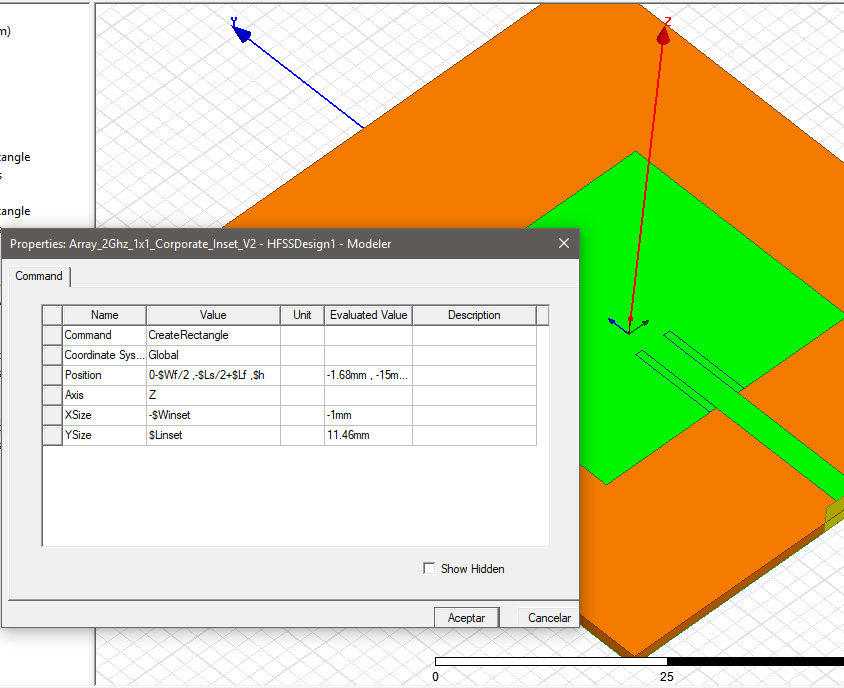
\includegraphics[width=\textwidth]{archivos/desarrollo/7a}
         \caption{Creación del \textit{inset} izquierdo}
         \label{fig:inseta}
     \end{subfigure}
     \hfill
     \begin{subfigure}[b]{0.45\textwidth}
         \centering
         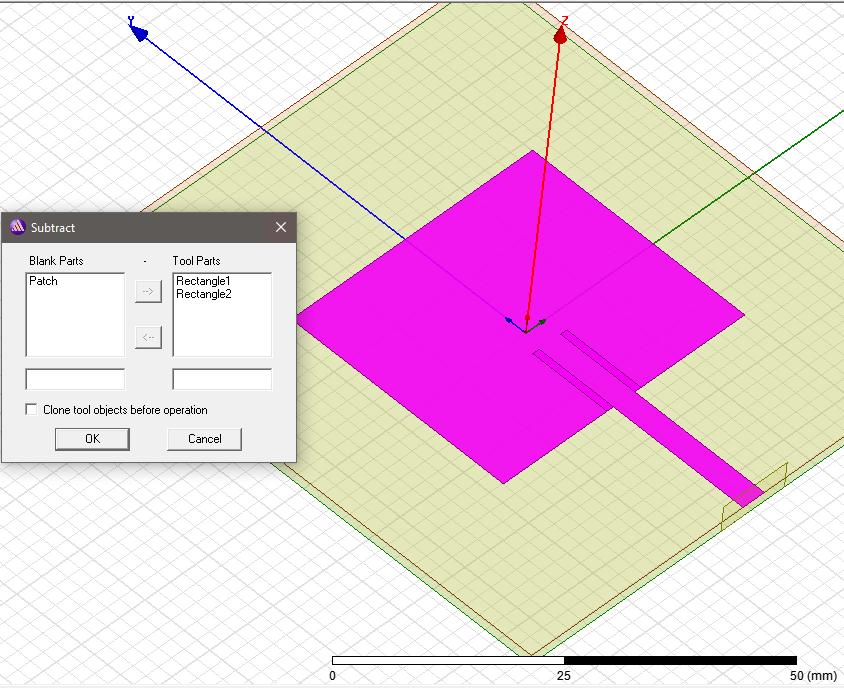
\includegraphics[width=\textwidth]{archivos/desarrollo/7b}
         \caption{Resta de la superficie de los \textit{insets}}
         \label{fig:insetb}
     \end{subfigure}
     \hfill
        \caption{Proceso de creación de los \textit{insets}}
        \label{fig:insets}
\end{figure}

\begin{figure}[h]
    \centering
        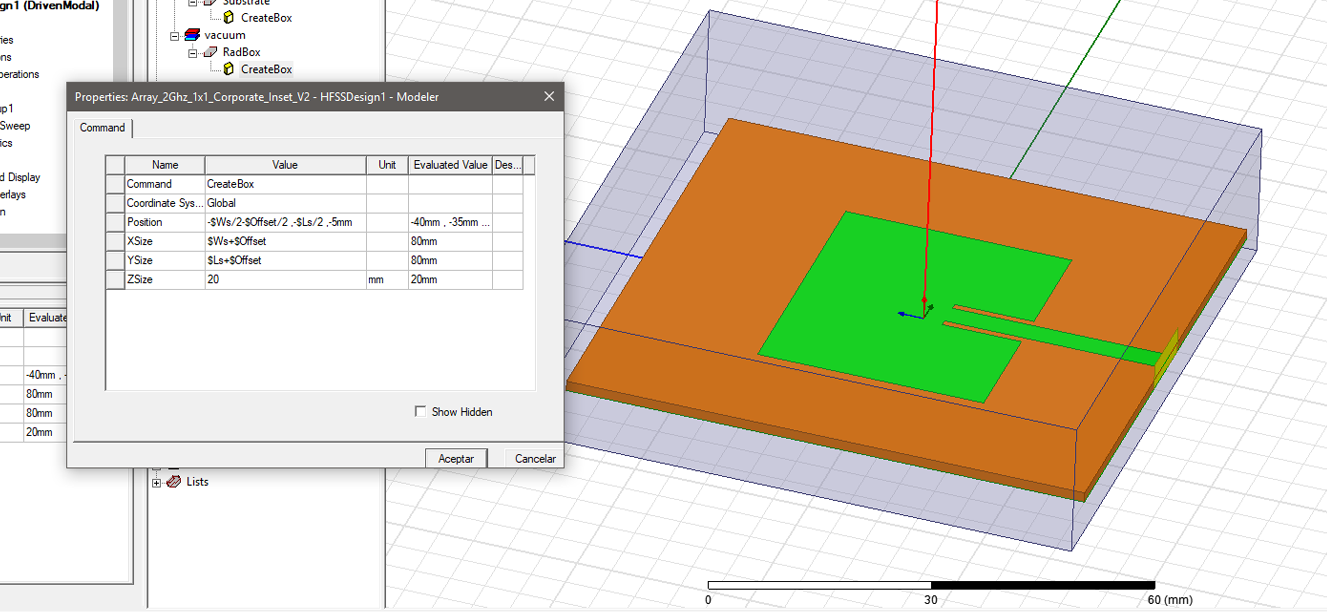
\includegraphics[width=13cm]{archivos/desarrollo/8}
        \caption{Creación del la caja de radiación}
        \label{fig:caja}
\end{figure}

\begin{figure}[H]
     \centering
     \begin{subfigure}[b]{0.48\textwidth}
         \centering
         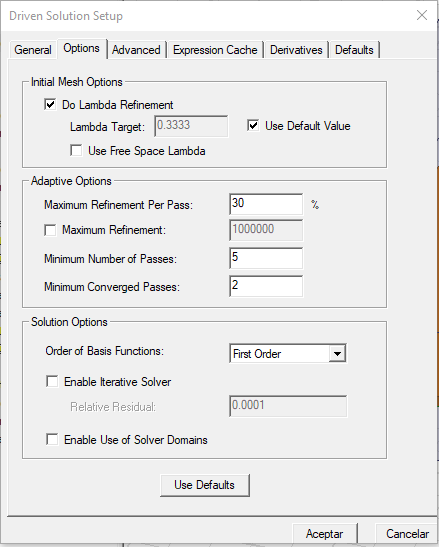
\includegraphics[width=\textwidth]{archivos/desarrollo/9a}
         \caption{Opciones de la configuración general}
         \label{fig:configa}
     \end{subfigure}
     \hfill
     \begin{subfigure}[b]{0.48\textwidth}
         \centering
         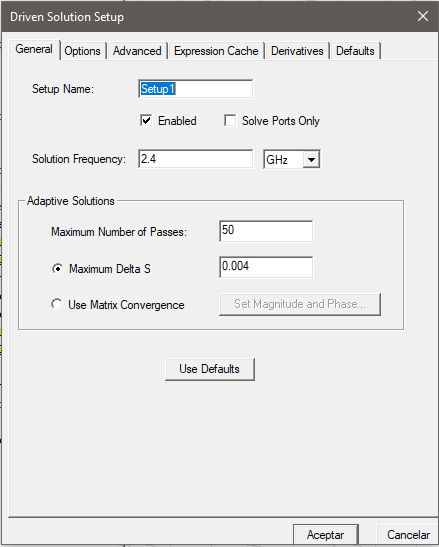
\includegraphics[width=\textwidth]{archivos/desarrollo/9b}
         \caption{Opciones de las iteraciones}
         \label{fig:configb}
     \end{subfigure}
     \hfill
     \\
     \begin{subfigure}[b]{0.48\textwidth}
         \centering
         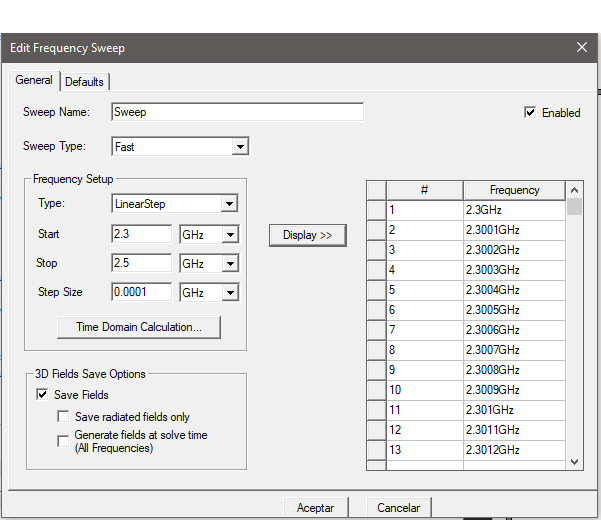
\includegraphics[width=\textwidth]{archivos/desarrollo/9c}
         \caption{Creación del barrido en frecuencia}
         \label{fig:configc}
     \end{subfigure}
     \hfill
        \caption{Configuración del simulador}
        \label{fig:config}
\end{figure}
\par El último elemento de diseño que se implementará será la caja de radiación. Esta se creará mediante la herramienta \textit{Draw box}, como se hizo con el substrato, y sus dimensiones deben ser capaces de cubrir el sistema entero que antena que se ha diseñado. Además, es importante el lado de la caja de radiación en el que se encuentra el \textit{Wave port} esté en el superpuesto en el plano de este (fig. \ref{fig:caja}). Además, de la misma forma que se hizo con elementos anteriores, se le asignará a este caja la propiedad de caja de radiación mediante: \textit{Assign Boundary}>\textit{Radiation} y como material: vacío.
\\
\par Llega el momento de configurar la simulación. Todas las opciones respecto a las iteraciones que va a realizar HFSS sobre el diseño se encuentran en la opción \textit{Analysis}, en sus opciones pulsaremos sobre \textit{Add Solution Setup}. En ella se introducirán los parámetros que se consideren necesarios para la correcta simulación del sistema. La frecuencia se ha establecido a 2.4 GHz \todo{fijarse en todos los GHz, todos lo que termine en "os", WavePorts}, el número máximo de pasadas como 50, y la máxima variación sobre el parámetro S de 0.004 (fig. \ref{fig:configa}). Si se entra a la pestaña \textit{options} se podrá también configurar parámetros como el número mínimo de pasadas, o el número mínimo de iteraciones consecutivas convergentes (fig. \ref{fig:configb}).
\\
\par Una vez creada la configuración del simulador, se añadirá el barrido en frecuencia sobre esta. Para ello, se añadirá un \textit{Frequency Sweep} mediante las opciones disponibles al pulsar sobre la configuración que hemos creado. En nuestro caso se configurará el barrido para crear un vector de frecuencias desde 2.3 GHz hasta 2.5 GHz cada 0.0001 GHz, creando un total de 1001 puntos de frecuencia para así obtener una mayor resolución en las gráficas que se deseen mostrar. El tipo de sweep se seleccionará como \textit{fast}, lo que ayudará a la máquina a agilizar el proceso de cálculo y es importante marcar la opción \textit{Save fields} para poder, más tarde, mostrar los datos relacionados con el campo lejano.
\\
\par Ya estaría listo el diseño y la configuración del solucionador para lanzar la simulación del sistema. Para ello se pulsará primero sobre el botón \textit{Validate} para confirmar que todo está correctamente configurado y no hay errores en el diseño que impidan que HFSS no pueda iniciar la simulación. Tras comprobar que no existen errores, mediante el botón \textit{Analyze all} se podrá iniciar la simulación. Durante la simulación HFSS irá realizando iteraciones en las que los tetraedros se irán adaptando a nuestro parche (fig. \ref{fig:tetra}). En cada iteración el número de tetraedros irá creciendo exponencialmente (fig. \ref{fig:conver}), con lo que es posible que en las últimas iteraciones, el simulador tarde más en realizar una pasada completa. Si se pulsa sobre la opción \textit{Convergence} dentro de las opciones del configurador de la simulación, se podrá obvservar de forma gráfica o anaítica el número de pasadas que ha realizado el simulador (fig. \ref{fig:convera}) así como otros datos sobre la convergencia de la simulación.
\\

\begin{figure}[H]
     \centering
     \begin{subfigure}[b]{0.47\textwidth}
         \centering
         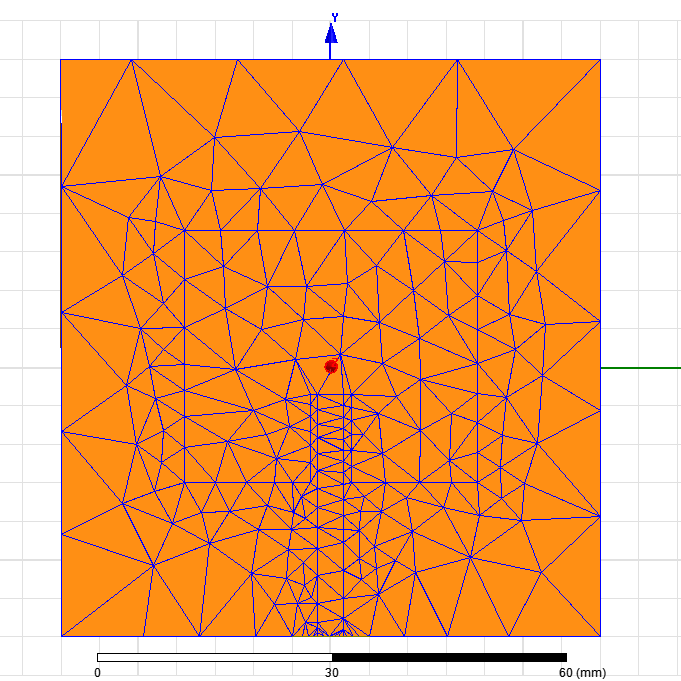
\includegraphics[width=\textwidth]{archivos/desarrollo/10a}
         \caption{Distribución de tetraedros en la iteración nº5}
         \label{fig:tetraa}
     \end{subfigure}
     \hfill
     \begin{subfigure}[b]{0.47\textwidth}
         \centering
         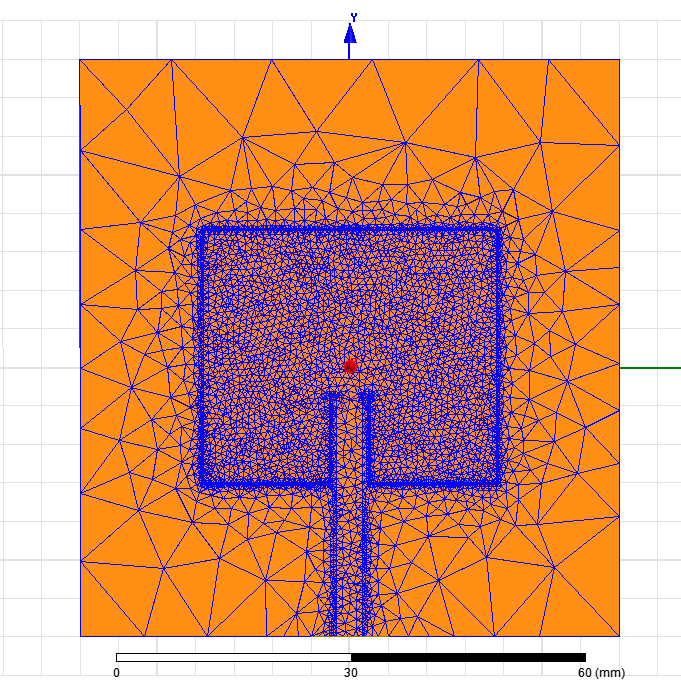
\includegraphics[width=\textwidth]{archivos/desarrollo/10b}
         \caption{Distribución de tetraedros en la iteración nº27}
         \label{fig:tetrab}
     \end{subfigure}
     \hfill
        \caption{Tetraedros creados por HFSS para calcular el comporamiento del sistema}
        \label{fig:tetra}
\end{figure}

\begin{figure}[H]
     \centering
     \begin{subfigure}[b]{0.47\textwidth}
         \centering
         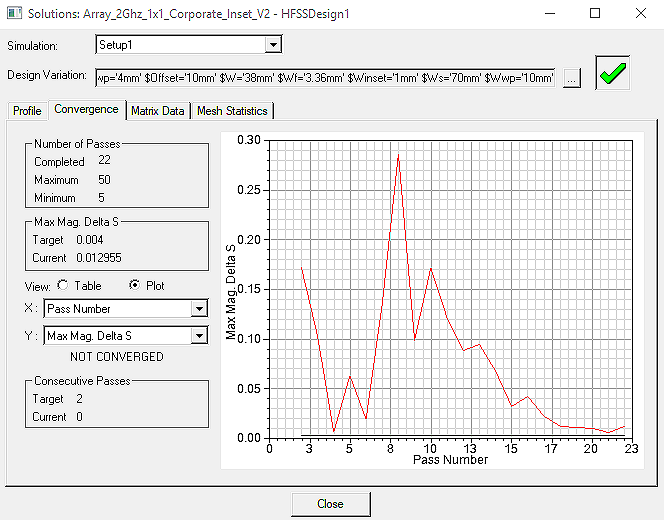
\includegraphics[width=\textwidth]{archivos/desarrollo/11a}
         \caption{Histórico de \textit{Delta S}}
         \label{fig:convera}
     \end{subfigure}
     \hfill
     \begin{subfigure}[b]{0.47\textwidth}
         \centering
         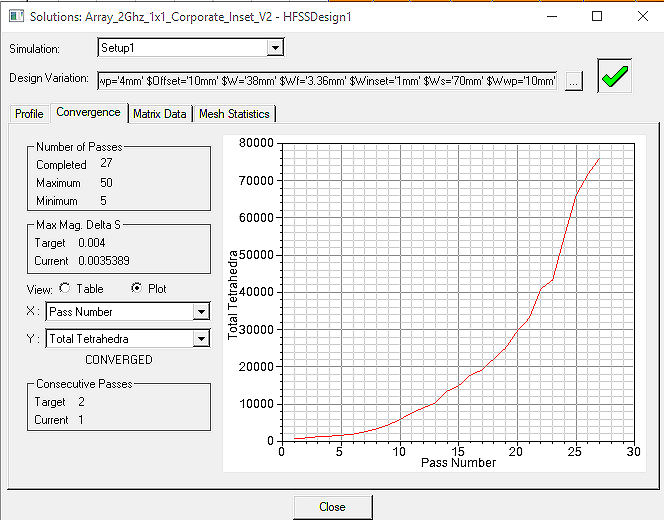
\includegraphics[width=\textwidth]{archivos/desarrollo/11b}
         \caption{Numero de tetraedros en la iteración nº27}
         \label{fig:converb}
     \end{subfigure}
     \hfill
        \caption{Datos sobre la simulación actual}
        \label{fig:conver}
\end{figure}

\par Una vez que la simulación ha convergido, HFSS empezará con otra serie de cálculos. Principalmente cálculos matriciales relacionados con los datos obtenidos de la simulación. Tras su finalización, se podrá proceder a analizar los resultados. Las gráficas de los resultados se obtienen mediante la pestalla \textit{Results}. Allí, al pulsar sobre sus opciones, se podrán acceder a diferentes tipos de representaciones según la naturaleza de esta: Reportes sobre soluciones modales, reportes sobre el campo lejano, etc. En primer lugar se analizará la curva de pérdida de retorno, o parámetro S, que se puede encontrar dentro de: \textit{Create Modal Solution Data Report}>\textit{Rectángular Plot}. Se abrirá una ventana donde se podrá seleccionar qué parámetro se quiere graficar, en nuestro caso \textit{S Parameter} en dB. En la misma ventana y dentro de la pesataña \textit{Families} se podrá seleccionar qué variación de nuestro diseño se quiere graficar, en el caso de que se hayan realizado más de una simulación con cambios en el diseño entre ellas. Finalmente, se pulsará sobre \textit{New Report} para ver el resultado.
\\
\par Como se mencionó al final de la sección \ref{351} Los resultados obtenidos mediante las dimensiones proporcionadas por las ecuaciones que se implementaron en MATLAB han de ser refinados, ya que estos no harán que nuestra antena funcione exactamente de la manera en la que se desea. Es necesario un trabajo previo al resultado final, basado en iteraciones propias realizadas por el ingeniero, en las que se modifiquen ciertas dimensiones de la antena para encontrar la solución que este busque. En el caso de esta antena, los resultados obtenidos tras el trabajo previo, en el que se han reducido 2 mm el ancho de la antena, se pueden ver a continuación. Cabe mencionar que, a lo largo del análisis de los resultados de nuestros diseños, se omitirá este proceso de refinado del diseño, y se mostrarán directamente las dimensiones con las que se ha encontrado que la antena trabaja según las especificaciones deseadas.
\\
\begin{itemize}
\item \textbf{Gráfica de pérdidas de retorno o parámetro S: }Se puede observar un buen comportamiento de la antena, con unas pérdidas de retorno en la frecuencia de trabajo de 2.4 GHz de -39.53 dBs, suficiente para el correcto funcionamiento de la antena a esta frecuencia, así como un ancho de banda a -10 dBs de de 36.5 MHz, lo que equivale a un 1.56\% sobre la frecuencia de trabajo.
	\begin{figure}[H]
    \centering
        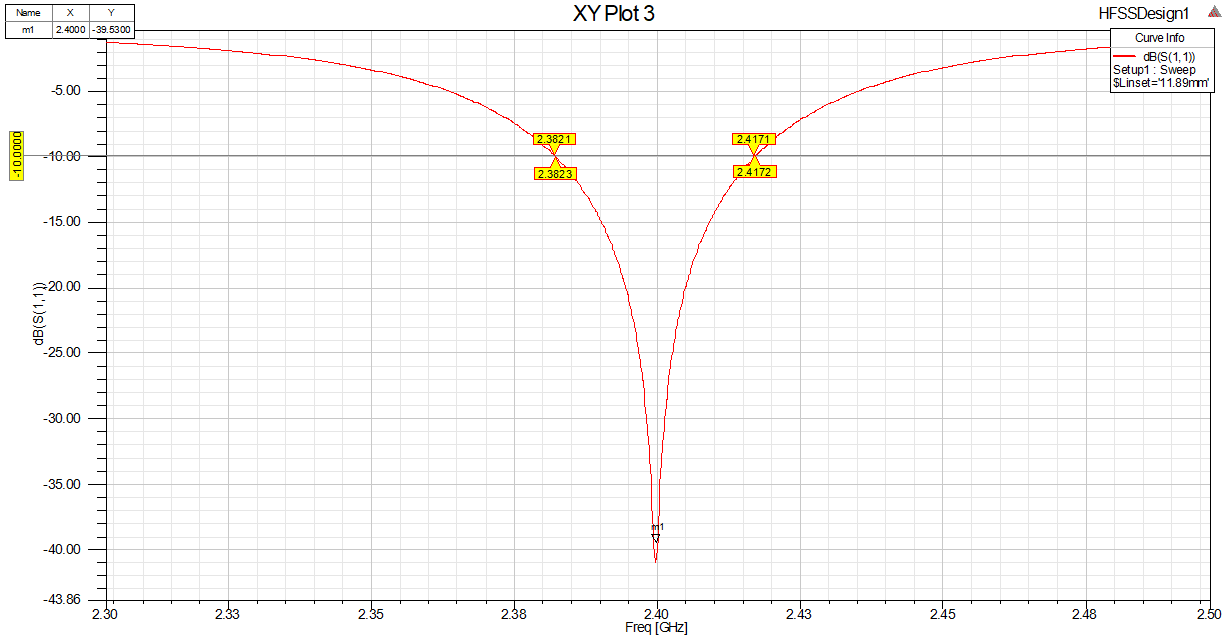
\includegraphics[width=14cm]{archivos/desarrollo/12a}
        \caption{Pérdidas de retorno}
        \label{fig:s}
	\end{figure}
	
\item \textbf{Gráfica del componente real de la impedancia: }En esta gráfica el objetivo principal es encontrar un valor de 50 $\Omega$ para la frecuencia de trabajo de 2.4 GHz. Este valor influencia directamente a la curva del parámetro S. Como se puede observar, el valor obtenido de 51 $\Omega$ lo que significa que la adaptación final entre el sistema de alimentación y la antena ha sido correcta.
	\begin{figure}[H]
    \centering
        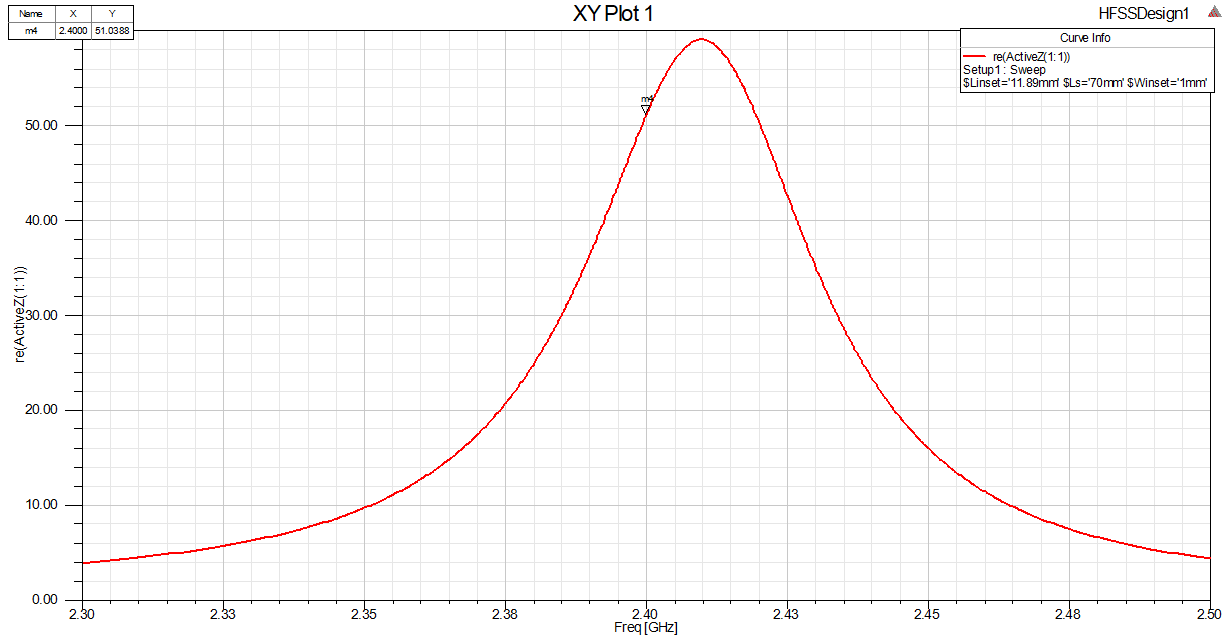
\includegraphics[width=14cm]{archivos/desarrollo/12b}
        \caption{Componente óhmica de la impedancia}
        \label{fig:realimpe}
	\end{figure}
	
\item \textbf{Gráfica del componente imaginaria de la impedancia: }En este caso, el cometido es encontrar un nulo de la curva de la componente reactiva de la impedancia para la frecuencia de trabajo. El valor obtenido para este diseño es de 0.23 $\Omega$, lo que puede considerarse como un buen resultado en el diseño.
	\begin{figure}[H]
    \centering
        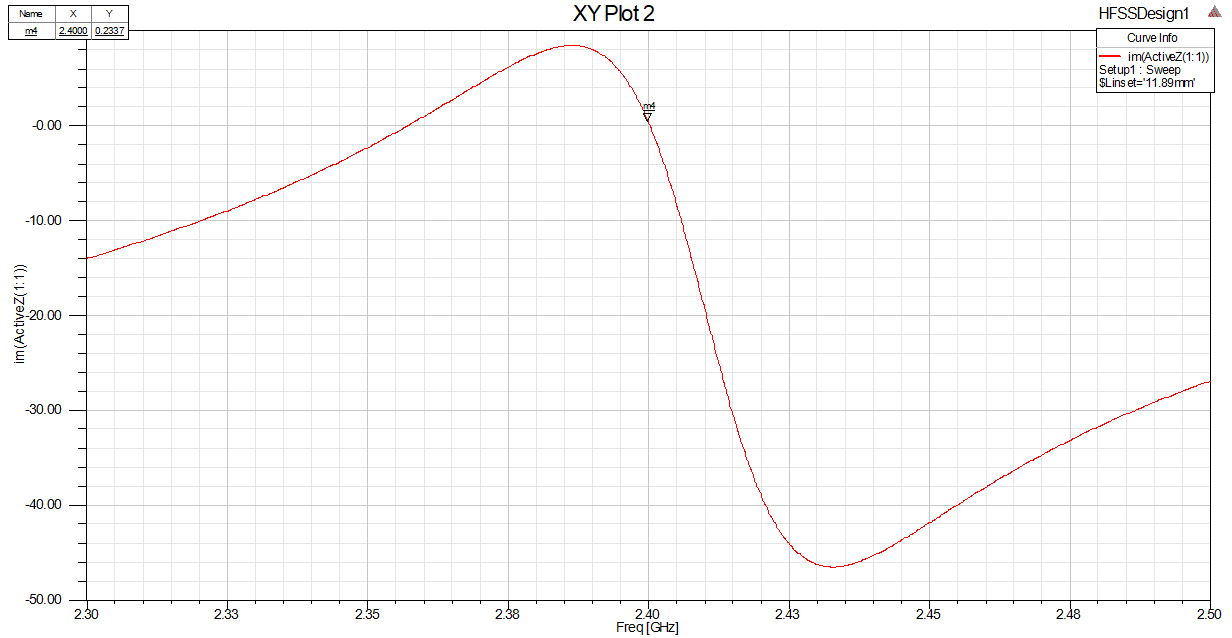
\includegraphics[width=14cm]{archivos/desarrollo/12c}
        \caption{Componente reactiva de la impedancia}
        \label{fig:imaimpe}
	\end{figure}

\item \textbf{Patrón de radiación en el plano E: }El patrón de radiación para el plano E, es aquel en el que se cumple que $\phi $ = 0º. En concreto el patrón de radiación que se mostrará a lo largo del proyecto es el correspondiente al de la directividad de la antena, medido en decibelios y en forma polar. Como se puede comprobar, el resultado obtenido es un patrón de radiación omnidireccional a lo largo del plano superior de la antena y un pequeño lóbulo trasero en el plano inferior. La directividad máxima de la antena, donde $\Theta$ = 0/360º, es de 5.36 dB. 
	\begin{figure}[H]
    \centering
        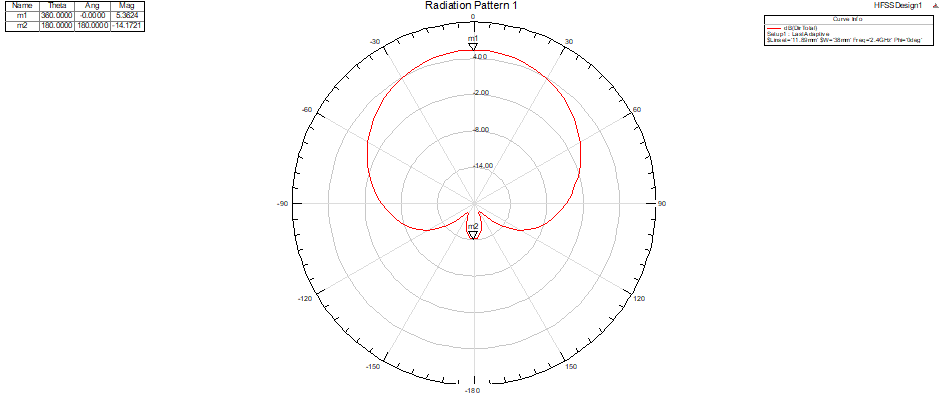
\includegraphics[width=14cm]{archivos/desarrollo/12d}
        \caption{Patrón de radiación del plano E}
        \label{fig:radE}
	\end{figure}

\item \textbf{Patrón de radiación en el plano H: }Repetiremos el proceso seguido para obtener el patrón de radiación en el plano E, pero con la principal diferencia de que el plano H es perpendicular a este, es decir, $\phi $ = 90º. Al tratarse de un parche único, no influenciado por otras antenas, el patrón de radiación en este plano es muy parecido al obtenido en la componente eléctrica, con una pequeña variación en la parte derecha del plano superior, producido por efectos conductores en la línea de alimentación microstrip. La directividad máxima obtenida en este plano es de 5.36 dB.
	\begin{figure}[H]
    \centering
        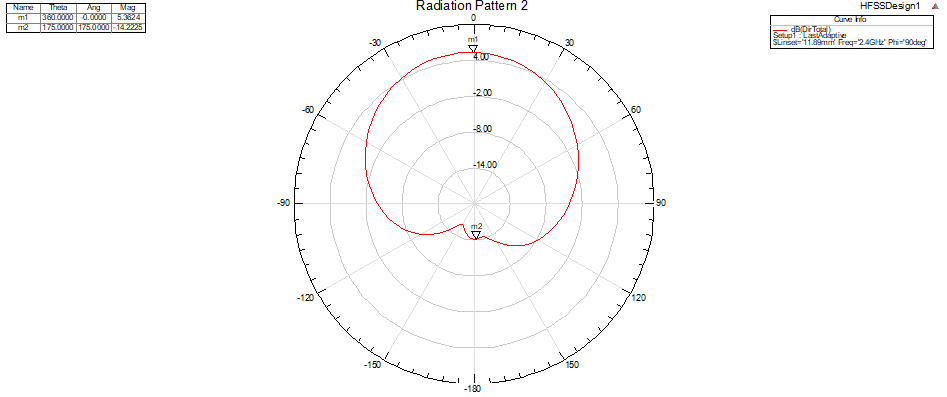
\includegraphics[width=14cm]{archivos/desarrollo/12e}
        \caption{Patrón de radiación del plano H}
        \label{fig:radH}
	\end{figure}

\item \textbf{Patrón de radiación tridimensional: }Aunque hemos mostrado los patrones de directividad para los ángulos $\phi $ en 0º y 90º, HFSS los calcula para la circunferencia completa. Se puede recrear el patrón de radiación en trews dimensiones si representamos juntos los patrones de dirección para todos los ángulos de $\phi$ y $\Theta$. HFSS ofrece una manera sencilla de hacerlo. Como se puede observar en los resultados, hemos obtenido una antena completamente omnidireccional para el plano superior del parche y una directividad casi nula en el plano inferior, lo que podríamos asimilar a un monopolo. La directividad obtenida siempre coincidirá con uno de los máximos, del campo E o H, en este caso 5.36 dB.
	\begin{figure}[H]
    \centering
        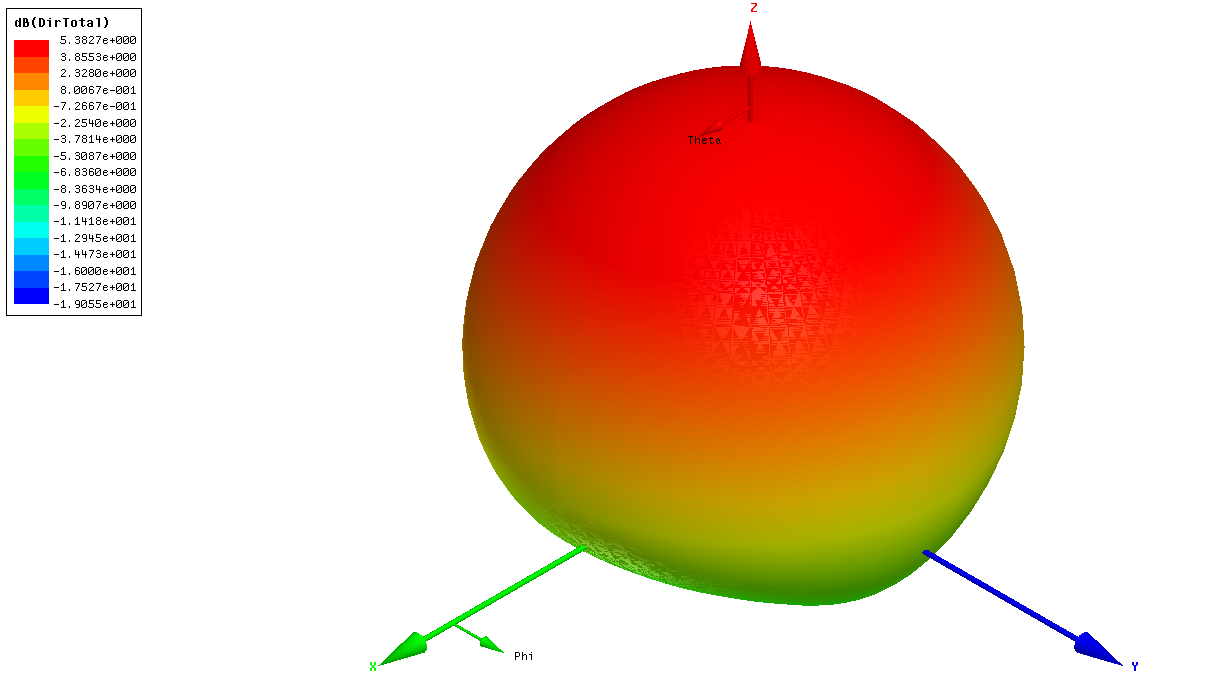
\includegraphics[width=14cm]{archivos/desarrollo/12f}
        \caption{Patrón de radiación 3D}
        \label{fig:rad3d}
	\end{figure}
	
\item \textbf{Distribución eléctrica sobre la antena: }Otro tipo de análisis que podemos realizar sobre la antena consiste en la muestra directa sobre la antena de ciertos parámetros como el campo eléctrico, los vectores de los campos eléctricos y magnéticos, etc. En este caso, se muestra la distribución del campo eléctrico sobre la antena. En el se pueden observar donde se sitúan los principales valles y nodos sobre esta.
	\begin{figure}[H]
    \centering
        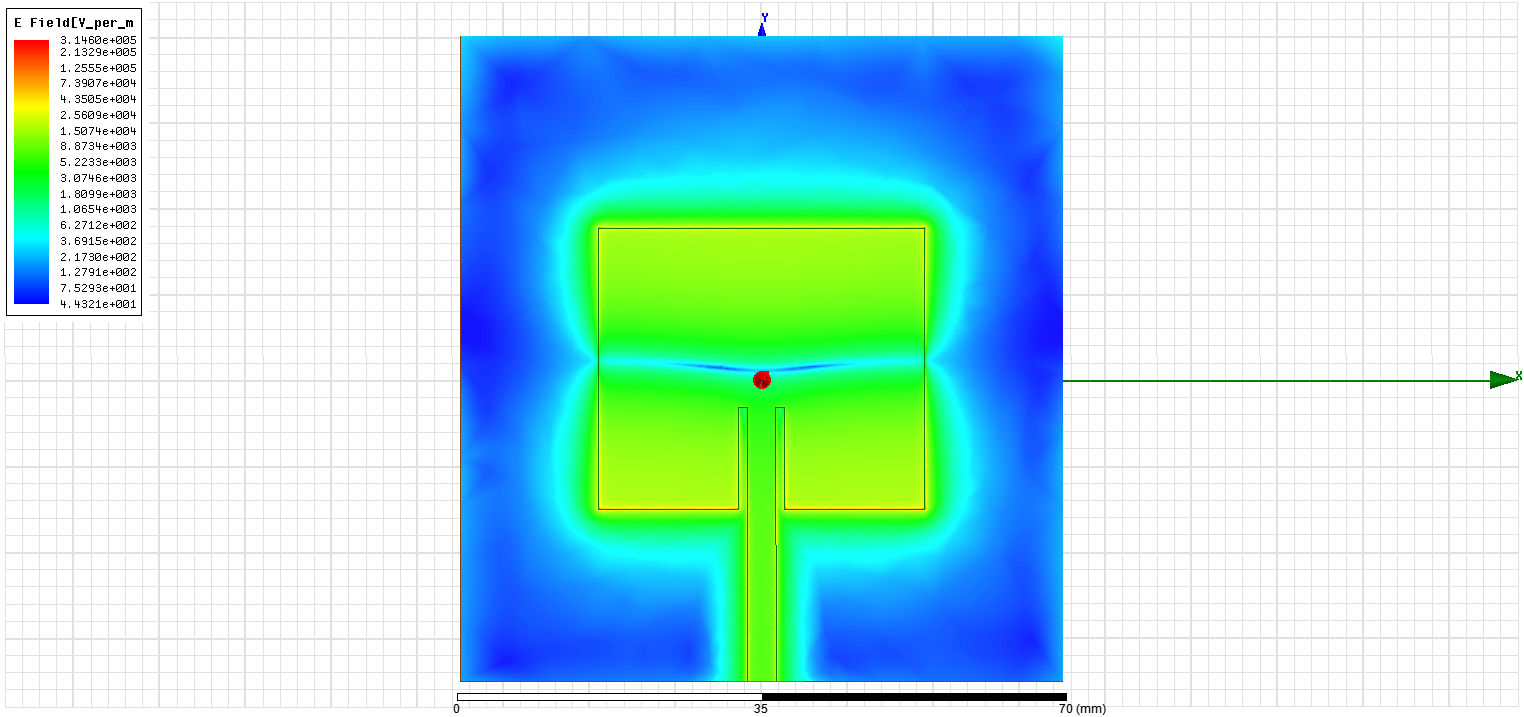
\includegraphics[width=14cm]{archivos/desarrollo/12g}
        \caption{Campos eléctricos en la superficie de la antena}
        \label{fig:Complexmage}
	\end{figure}

\end{itemize}
